%% Document class
\documentclass[final,3p,times,onecolumn]{elsarticle}    % one column normal format
%\documentclass[preprint,review,12pt]{elsarticle}        % one column review format

%% Use package
\usepackage{graphicx}
\usepackage{epstopdf}
\usepackage{amssymb}
\usepackage{amsthm}
\usepackage{amsmath}
\usepackage{latexsym}
\usepackage{mathrsfs}
\usepackage[tight,nice]{units}
\usepackage{harpoon}
\usepackage{chemarrow}
\usepackage{lineno}
\usepackage{harpoon}
\usepackage{chemarrow}
\usepackage{lscape}
\usepackage{color}
\usepackage{lineno}
\usepackage{colortbl}
\usepackage{chngcntr}
\usepackage{etoolbox}
\usepackage{tikz}
\usepackage{float}
\usepackage{soul}
\usepackage{xr}

%% Uncomment if no abstract
\usepackage{xpatch}
\xpatchcmd{\MaketitleBox}{\hrule}{}{}{}
\xpatchcmd{\MaketitleBox}{\hrule}{}{}{}

%% Bib options
\biboptions{sort&compress}

%% Cross referencing option
\makeatletter
\newcommand*{\addFileDependency}[1]{
    \typeout{(#1)}
    \@addtofilelist{#1}
    \IfFileExists{#1}{}{\typeout{No file #1.}}  }

\makeatother
\newcommand*{\myexternaldocument}[1]{
    \externaldocument{#1} 
    \addFileDependency{#1.tex} 
    \addFileDependency{#1.aux}  }

\myexternaldocument{main}

%% Figure and table S prefix
\renewcommand{\thefigure}{S\arabic{figure}}
\renewcommand{\thetable}{S\arabic{table}}
\renewcommand{\theequation}{S\arabic{equation}}

%% Eliminates automatic footer note
\makeatletter
\def\ps@pprintTitle{%
  \let\@oddhead\@empty
  \let\@evenhead\@empty
  \let\@oddfoot\@empty
  \let\@evenfoot\@oddfoot
}

%% Begin document
\begin{document}

%%%%%%%%%%%%%%%%%%%%%%%%%%%%%%%%%%%%%%%%%%%%%%%%%%%%%%%%%%%%%%%%%%%%%%%%%%
%% Begin Frontmatter
\begin{frontmatter}
\title{Supplementary Information: Predicted Impacts of Pt and Ionomer Distributions \\ 
       on Low Pt-loading PEMFC Performance}

\author[CSM]{Corey R. Randall}
\author[CSM]{Steven C. DeCaluwe \corref{cor}}
\cortext[cor]{Corresponding Author: Tel: (303) 273-3666}
\ead{decaluwe@mines.edu}
% \author[org1name,org2name]{Another Author}
        
\address[CSM]{Colorado School of Mines, 1500 Illinois St, Golden, CO 80401}
% \address[org2name]{org2 name, org2 address}
\end{frontmatter}

%%%%%%%%%%%%%%%%%%%%%%%%%%%%%%%%%%%%%%%%%%%%%%%%%%%%%%%%%%%%%%%%%%%%%%%%%%
\section{Geometric parameters}

\begin{figure}[H]
    \centering
    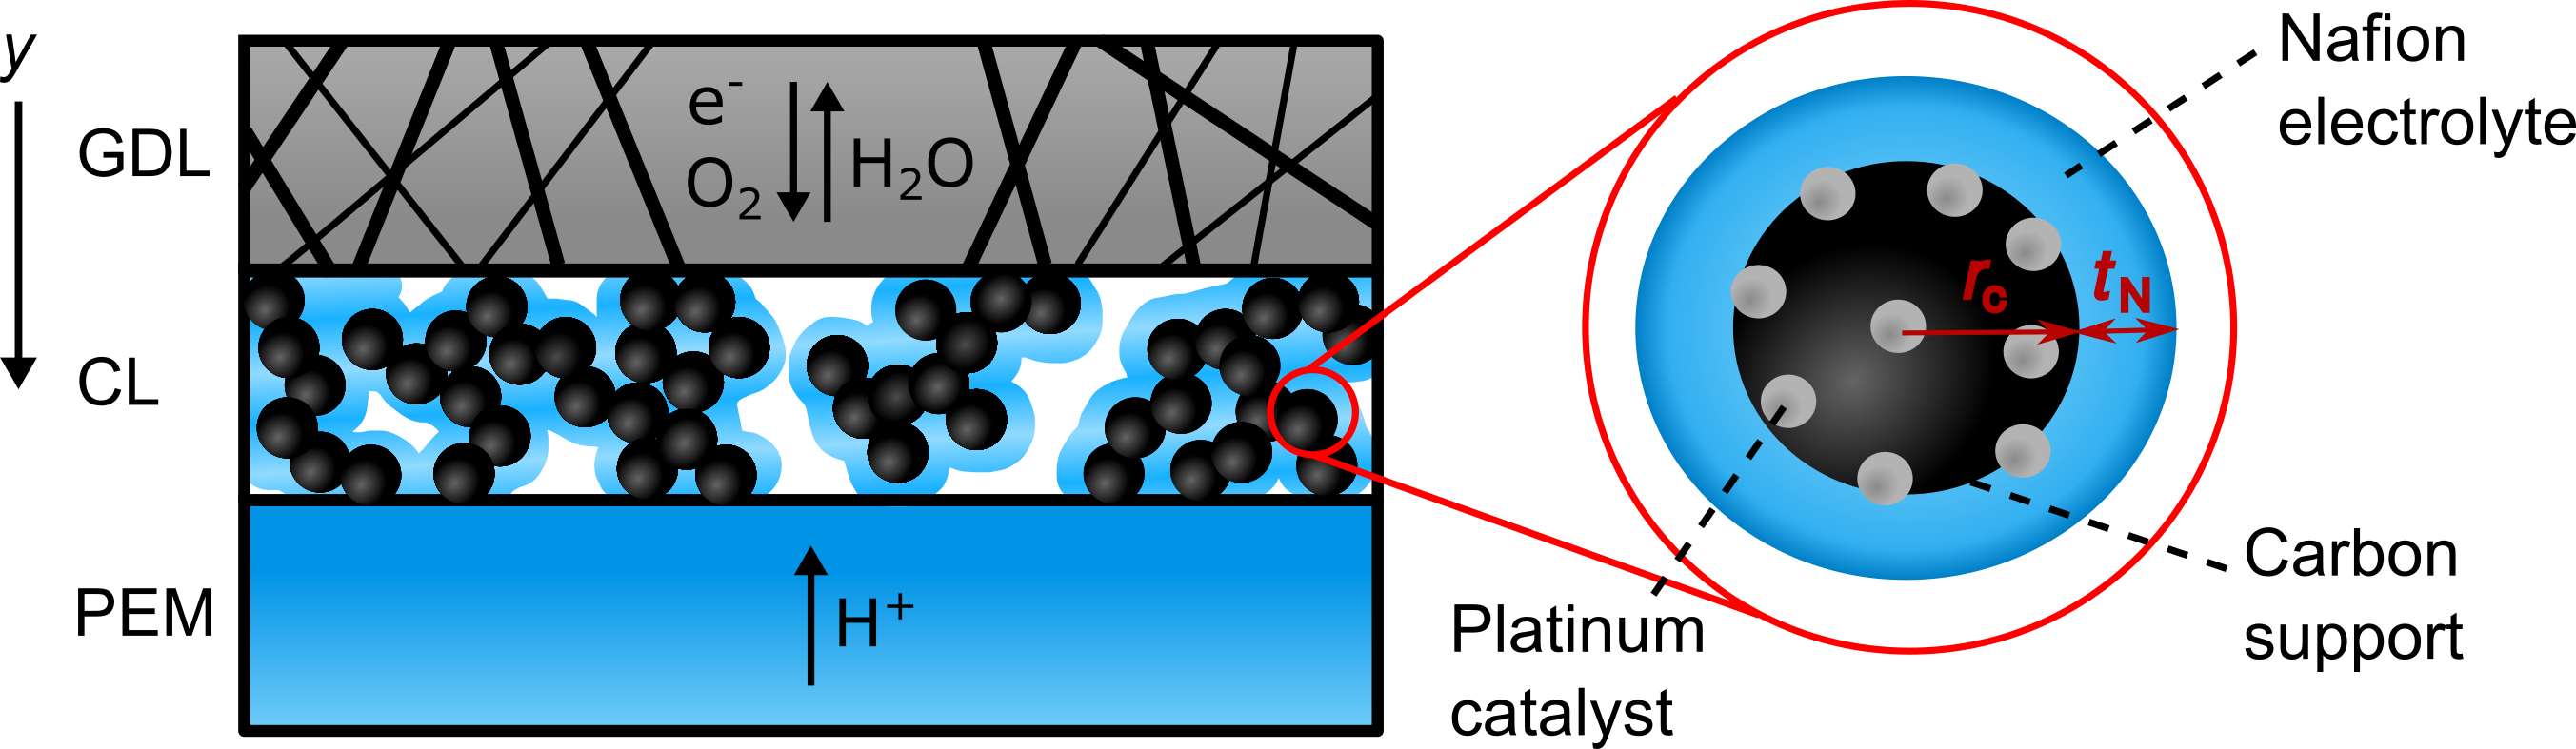
\includegraphics[width=5.718in]{figures/core_shell_SI.png}
    \caption{Illustration of the model domain. The catalyst layer consists entirely of Nafion-coated, Pt-decorated carbon nanoparticles.  The representative `core-shell' particle is assumed spherical, as shown in the call-out. The total radius of this representative particle equals the sum of the carbon radius $r_c$ and the Nafion shell thickness $t_{\rm N}$}
    \label{fig:core_shell_SI}
\end{figure}

This model includes numerous parameters, some of which are difficult to estimate directly from scanning electron microscope or transmission electron microscope images. For example, the reaction surface areas, defined as m$^2$ per m$^3$ of total volume, are not readily available. For this model, these areas and other parameter are derived using a minimal number of geometric inputs, shown in table~\ref{tab:geometry}, which are more readily attained from imaging catalyst layers.

\begin{table}[!htb]
    \centering
    \caption{Geometric parameters}
    \begin{tabular}{l c c}
    \hline \hline
    Parameter                       &Value      &Units  \\
    \hline
    Carbon radius ($r_{\rm c}$)     &50         &nm     \\
    Nafion thickness ($t_{\rm N}$)  &12         &nm     \\
    CL thickness ($t_{\rm CL}$)     &15         &$\mu$m \\
    GDL thickness ($t_{\rm GDL}$)   &250        &$\mu$m \\
    Pt radius ($r_{\rm Pt}$)        &1          &nm     \\
    Dry CL porosity ($\epsilon_{\rm g,CL}^{\circ}$)   &0.1    &[-] \\
    Dry GDL porosity ($\epsilon_{\rm g,GDL}^{\circ}$)  &0.5    &[-] \\
    \hline \hline
    \end{tabular}
    \label{tab:geometry}
\end{table}

\subsection{Basic calculations}
As shown in Figure~\ref{fig:core_shell_SI}, we assume that the representative Nafion-coated, Pt-decorated carbon particle in each volume is spherical. The solid volume of a single core-shell particle (a carbon `core' coated with a Nafion `shell') is therefore calculated as
\begin{equation}\label{eq:V_solid}
    V_{\rm solid} = \frac{4}{3} \pi (r_{\rm c} + t_{\rm N})^3,
\end{equation}
where $r_{\rm c}$ and $t_{\rm N}$ are the carbon particle radius and Nafion shell thickness. The surface area of the same particle is
\begin{equation}
    A_{\rm solid} = 4 \pi (r_{\rm c} + t_{\rm N})^2. 
\end{equation}
The Nafion-water, Nafion-gas, and water-gas rection areas per core-shell particle are proportional to this $A_{\rm solid}$ value, as described in the main body of the manuscript:
\begin{equation}
    A_{\rm rxn,\,N-g} = (1-{\cal S}_w)\,A_{\rm solid}.
\end{equation}
and
\begin{equation}
    A_{\rm rxn,\,N-w} =A_{\rm rxn,\,w-g} =  {\cal S}_w\,A_{\rm solid},
\end{equation}
where ${\cal S}_w$ is the local water saturation. The Nafion volume for a single core-shell particle is the difference between the total particle volume and the volume of the carbon core,
\begin{equation}
    V_{\rm N} = \frac{4}{3} \pi (r_{\rm c} + t_{\rm N})^3 - \frac{4}{3} \pi r_{\rm c}^3.
\end{equation}
The surface area of the carbon core is used to approximate the double layer area. For a single particle, it is
\begin{equation}
    A_{\rm rxn,\,dl} = 4 \pi r_{\rm c}^2.
\end{equation}

\subsection{Specific reaction areas}
The model takes the dry porosity ($\epsilon_{\rm g,CL}^{\rm o}$) as an input parameter. This means that the volume fraction of solid (i.e. carbon, Pt, and Nafion) is $1 - \epsilon_{\rm g,CL}^{\rm o}$. To obtain any specific area ($A_{i}^{\prime\prime\prime}$, m$^2$ m$^{-3}_{\rm tot}$), the following conversion is used
\begin{equation} \label{eq:specific-rxn-areas}
    A_{i}^{\prime\prime\prime} 
    = \frac{A_{\rm i,\,rxn}}{V_{\rm solid}} \frac{V_{\rm solid}}{V_{\rm total}} 
    = \frac{A_{\rm i,\,rxn}}{V_{\rm solid}} (1 - \epsilon_{\rm g,CL}^{\rm o}),
\end{equation}
where $i$ is one of `N-g',  `N-w', `w-g', or `dl', and $V_{\rm solid}$ is as calculated in equation~\ref{eq:V_solid}. The triple prime notation used here denotes that areas are per unit volume. The prime symbols are neglected in the main manuscript to reduce the notation complexity, but are presented here for rigor and clarity. 

For the specific Pt surface area, the Pt loading ($w_{\rm Pt}$, g$_{\rm Pt}$m$^{-2}$) is needed. If  Pt is uniformly distributed, then the overall Pt density in the catalyst layer is
\begin{equation}\label{eq:rho_pt_cl}
    \rho_{\rm Pt, CL} = \frac{w_{\rm Pt}}{t_{\rm CL}},
\end{equation}
where $t_{\rm CL}$ is the catalyst layer thickness. When graded Pt distributions are considered, the Pt loading is multiplied by a fraction taken from an arithmetic or geometric sequence, representing linear and exponential functions for Pt distribution, respectively. The local Pt density is then calculated using the local discretized CL volume thickness $t_i$, rather than the total catalyst layer thickness $t_{\rm CL}$ in equation~\ref{eq:rho_pt_cl}. To preserve the same total Pt loading as in a uniformly loaded cell, the arithmetic/geometric sequence fractions add to unity. The Pt catalyst is assumed to exist as half spheres with radius $r_{\rm Pt}$, resulting in an area and volume per half sphere of:
\begin{equation}
    A_{\rm Pt} = 2 \pi r_{\rm Pt}^2 \quad \textrm{and} \quad V_{\rm Pt} = \frac{2}{3} \pi r_{\rm Pt}^3.
\end{equation}
Combined with the density of pure Pt ($\rho_{\rm Pt}$), the specific surface area of Pt is calculated using these values as
\begin{equation}
    A_{\rm Pt}^{\prime\prime\prime} 
    = \frac{\rho_{\rm Pt, CL}}{\rho_{\rm Pt}} \frac{A_{\rm Pt}}{V_{\rm Pt}}.
\end{equation}

\subsection{Nafion volume fraction}
The factor used in equation~(\ref{eq:specific-rxn-areas}) can also be used to convert the volume of Nafion per particle to the total Nafion volume fraction, $\epsilon_{\rm N}$:
\begin{equation}
    \epsilon_{\rm N} = \frac{V_{\rm N}}{V_{\rm solid}} \frac{V_{\rm solid}}{V_{\rm total}}
                     = \frac{V_{\rm N}}{V_{\rm solid}} (1 - \epsilon_{\rm g,CL}^{\rm o}).
\end{equation}
We note here that although the Pt is represented by half spheres within the Nafion shell, the model is primarily run with low loadings and assumes $r_{\rm Pt} << r_{\rm c}$, supporting the assumption of sphericity for the overall core-shell domain. 

%%%%%%%%%%%%%%%%%%%%%%%%%%%%%%%%%%%%%%%%%%%%%%%%%%%%%%%%%%%%%%%%%%%%%%%%%%
\section{Supplementary figures}
Figures~\ref{fig:validation_o2}--~\ref{fig:Pt-distribution-study} present polarization and power density curves not reported in the main body of the manuscript.  Figure~\ref{fig:validation_o2} presents best fits of the model to validation data from Owejan, et. al~\cite{bib:owejan_2013} for an O$_2$-fed cathode.  These fits are for all three CL Nafion transport models.  The model provides a suitable qualitative fit for the `Uniform' and `Mixed' transport models.  However, especially compared to the air-fed cathode results in figure~\ref{fig:validation_air}, the model slightly under-predicts the difference between high and low Pt-loaded PEMFCs. It is likely that further refinement of model approaches or parameter estimates are required for a model that captures behavior of O$_2$-fed cells.  Possible improvements which would capture additional limiting phenomena include:
\begin{itemize}
    \item Elementary 2-step charge transfer reaction, rather than the global single-step reaction~\ref{eq:orr-2}.
    \item Experimentally-validated transport mechanism for O$_{\rm 2,\,N}$. THe current approach assumes, based on geometric analysis, that O$_{\rm 2,\,N}$ diffusion coefficients scale with the local Nafion water volume fraction.
    \item Experimentally-validated reaction rate coefficients for O$_2$ absorption in to Nafion.
\end{itemize}
\begin{figure}[H]
    \centering
    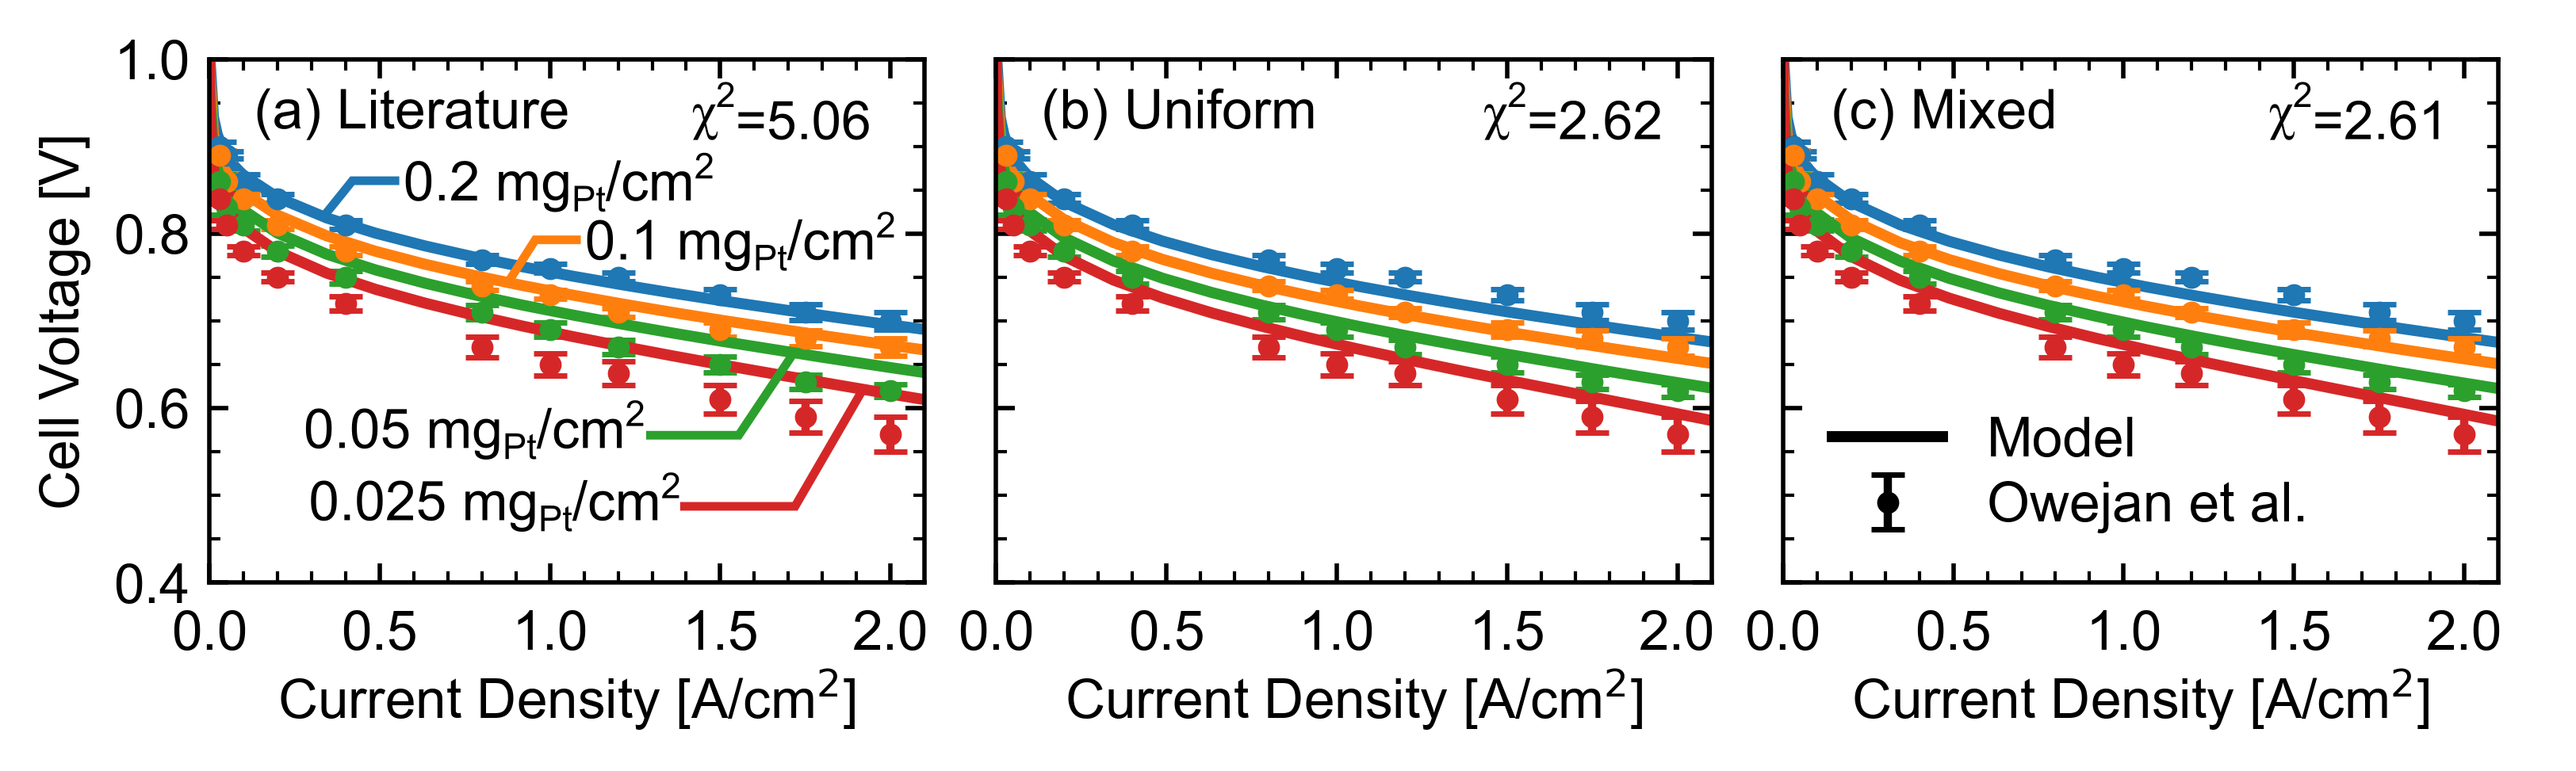
\includegraphics[width=6.47in]{figures/validation-o2-6_47in.png}
    \caption{Simulation results and experimental data~\cite{bib:owejan_2013} for oxygen-fed PEMFCs with varying Pt loading. Transport properties within thin-film Nafion are taken from (a) literature~\cite{bib:yadav_2012, bib:sethuraman_2009} and (b-c) structure-property relationships developed within this work. Differences between the (b) uniform and (c) mixed structure-property relationships are described in section~\ref{sect:struct-prop-relationships}.}
    \label{fig:validation_o2}
\end{figure}
Figure~\ref{fig:CL-thickness-study} shows polarization and power density curves for the air-fed PEMFC with varying CL thickness.  As mentioned in the manuscript, thinner CLs reduce ion transport lenths, leading to lower Ohmic overpotentials and higher max power densities.  However, as seen in figure~\ref{fig:CL-thickness-study}(b), the max power with decreasing CL thickness occurs closer and closer to the PEMFC limiting current.
\begin{figure}[H]
    \centering
    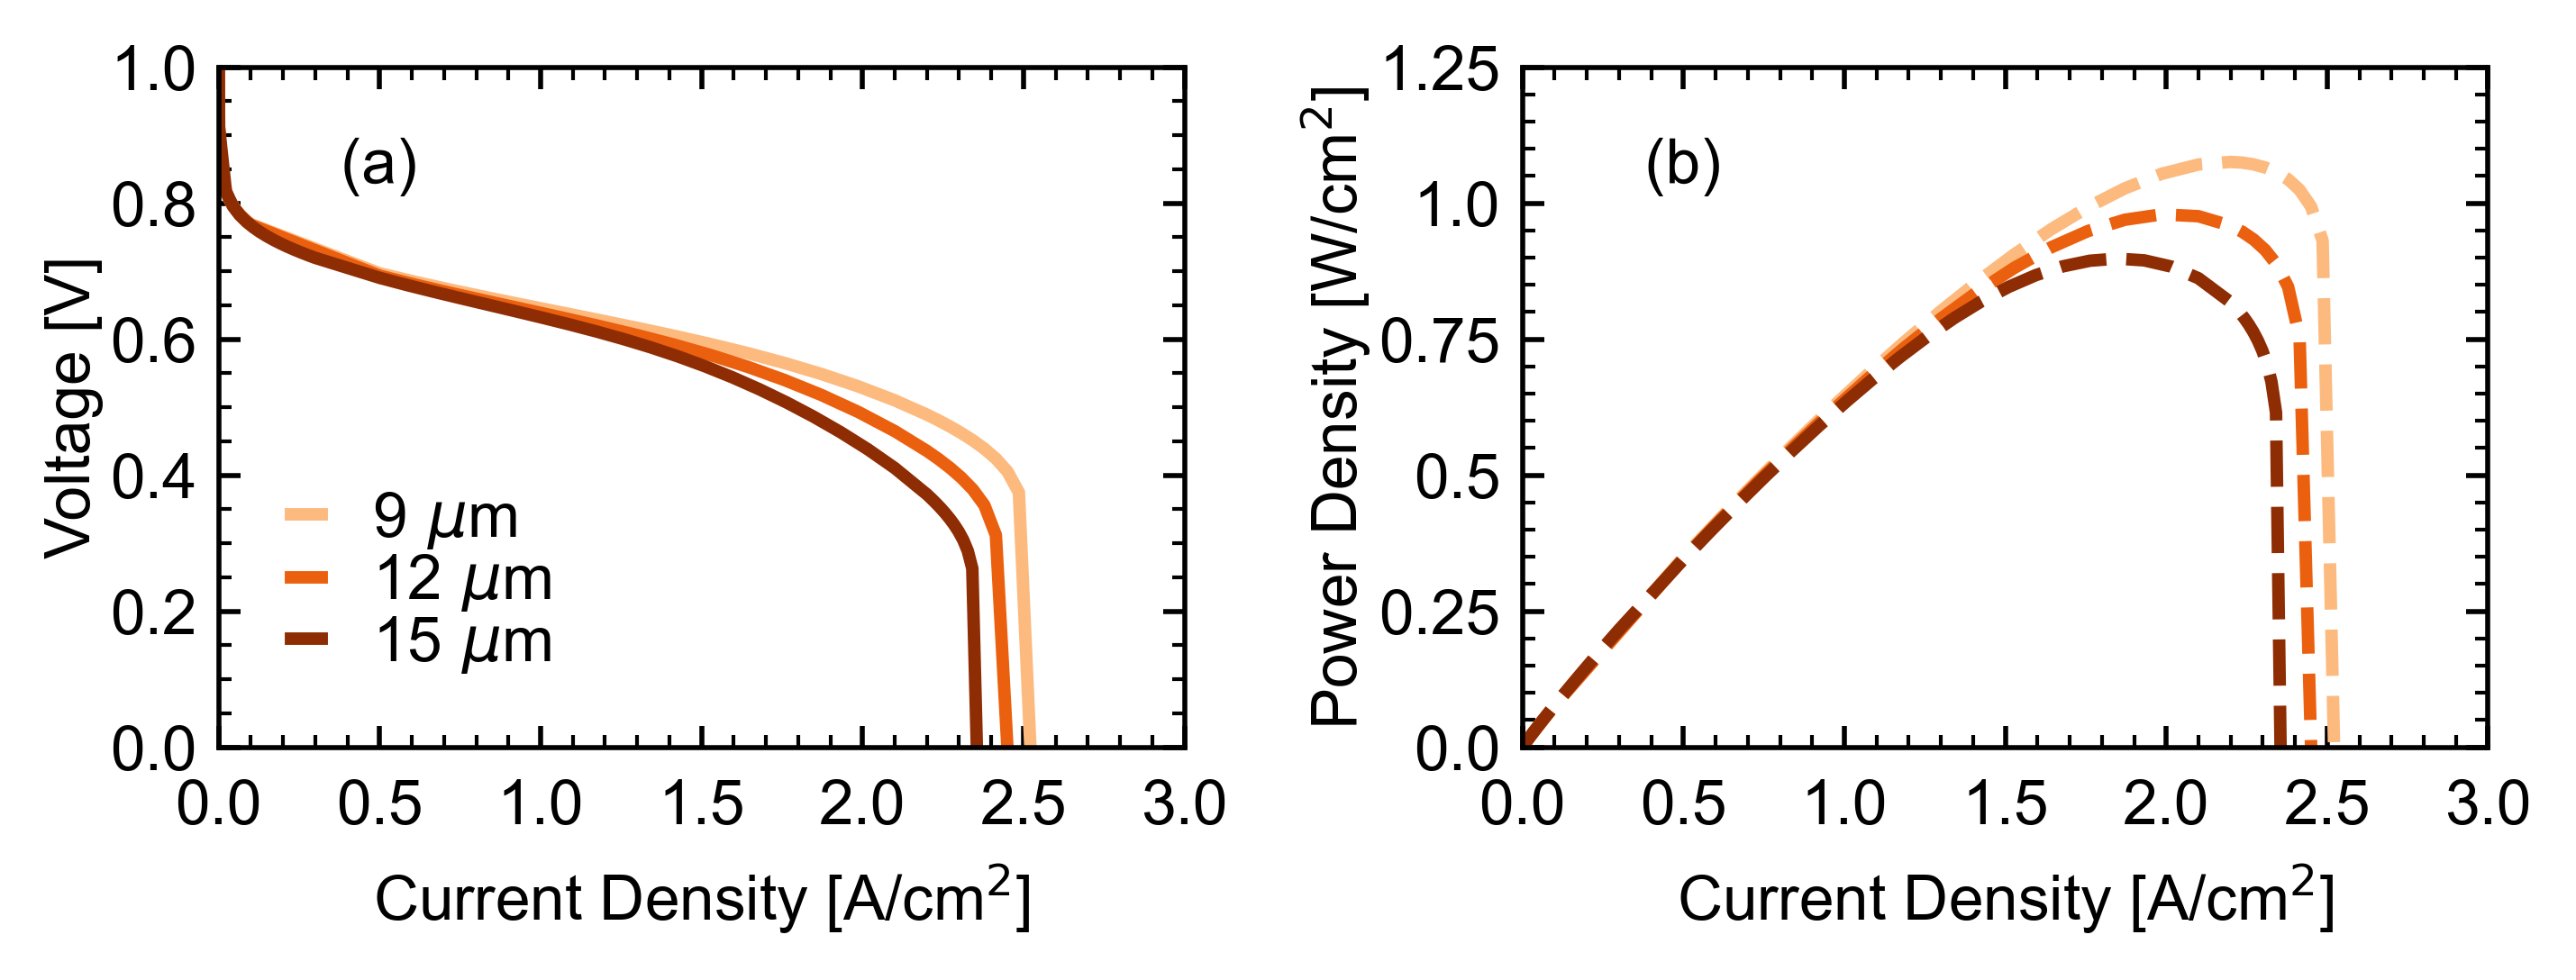
\includegraphics[width=5.718in]{figures/CL-thickness-5_718in.png}
    \caption{(a) Polarization and (b) power density curves for varying CL thicknesses. The 15~$\mu$m curves are from the model validation base case. Results suggest that thinner CLs improve performance, however, the maximum power density occurs closer to the limiting current.}
    \label{fig:CL-thickness-study}
\end{figure}
Figure~\ref{fig:naf-thickness-study} shows results for increasing Nafion shell thickness.  As noted in the manuscript, results indicate that improved performance with increased $\sigma_{\rm ion}^{\rm eff}$ outweigh any deleterious effects from increase O$_2$ transport lengths between the pore and Pt catalyst surface.  Moreover, losses due to transport through thickner Nafion are mitigated by the higher water volume fractions in these thicker films.
\begin{figure}[H]
    \centering
    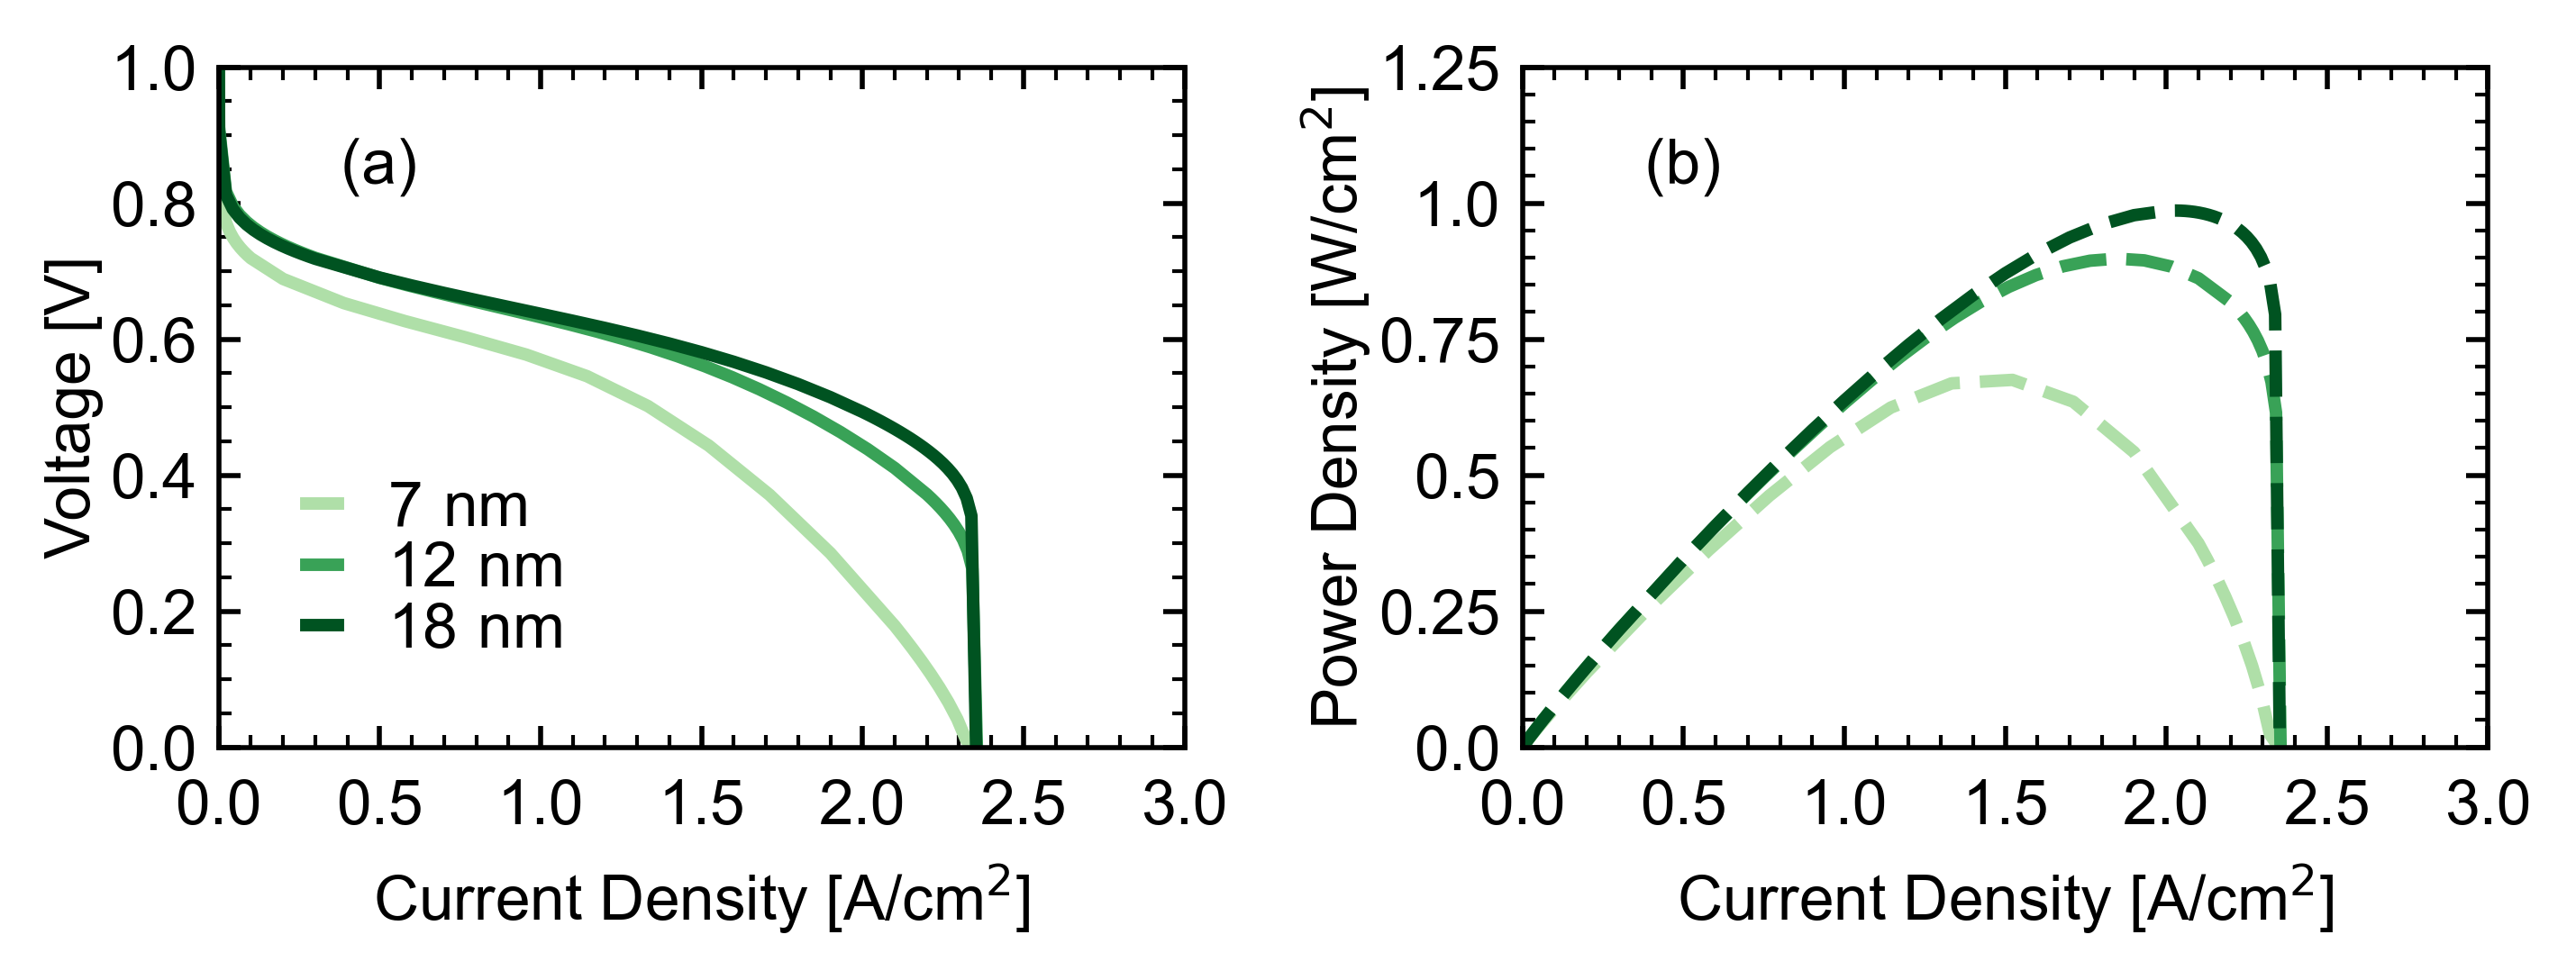
\includegraphics[width=5.718in]{figures/naf-thickness-5_718in.png}
    \caption{(a) Polarization and (b) power density curves for varying Nafion shell thicknesses. The 12~nm curves are from the model validation base case. Results suggest that when ionomer loading is uniform, thicker shells increase cell performance by lowering Ohmic resistance.}
    \label{fig:naf-thickness-study}
\end{figure}
\newpage
Figure~\ref{fig:naf-distribution-study} shows performance with varying Nafion thickness distributions as a function of CL depth. As noted in the manuscript, the Nafion loading mainly impacts the limiting current $j_{\rm lim}$, but has little impact on the maximum power density.
\begin{figure}[H]
    \centering
    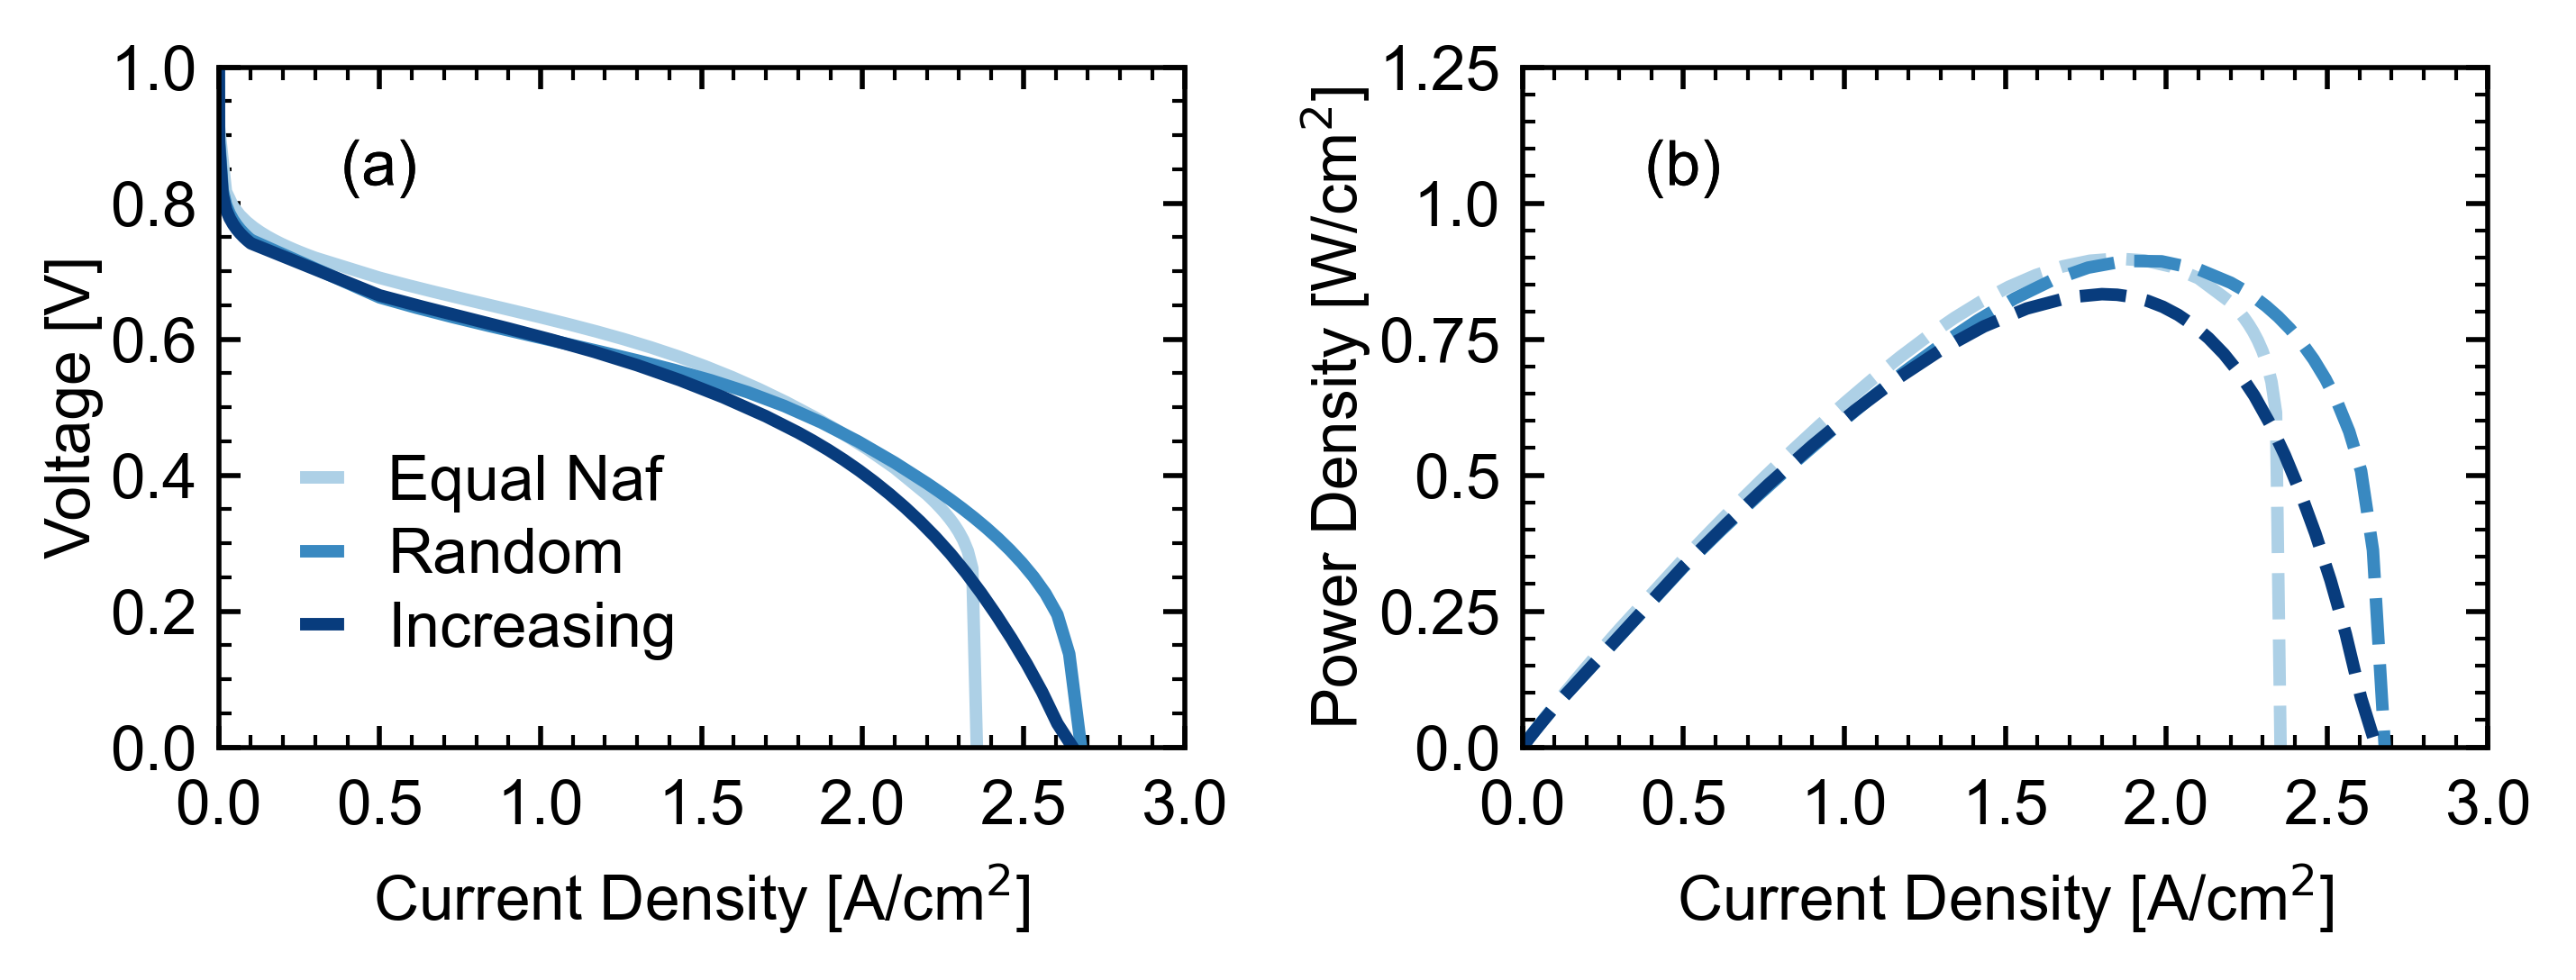
\includegraphics[width=5.718in]{figures/naf-distribution-5_718in.png}
    \caption{(a) Polarization and (b) power density curves for varying ionomer distributions. The curves labeled ``Equal Naf'' are for the model validation base case where the ionomer is evenly distributed. Results suggest that randomly distributed and linearly graded Nafion between the GDL and PEM interfaces can improve limiting currents by reducing flooding.}
    \label{fig:naf-distribution-study}
\end{figure}
Lastly, figure~\ref{fig:Pt-distribution-study} shows predicted performance for cells with varying Pt distributions.  All three cells have a total, integrated loading of 0.025 mg$_{\rm Pt}$ cm$^{-2}$.  For `Equal Pt,' the Pt is uniformly distributed throughout the CL.  The `Linear' and `Exponential' profiles are for cells where the Pt is concentrated closer to the PEM, as discussed above and in the manuscript.  In theory, concentrating Pt closer to the PEM should reduce Ohmic losses and lead to higher maximum power.  While we see slight increases to the maximum power density with non-uniform Pt distributions, these gains are negligible, especially when one considers the concomitant decreases in the limiting currents, due to flooding effects in the CL.
\begin{figure}[H]
    \centering
    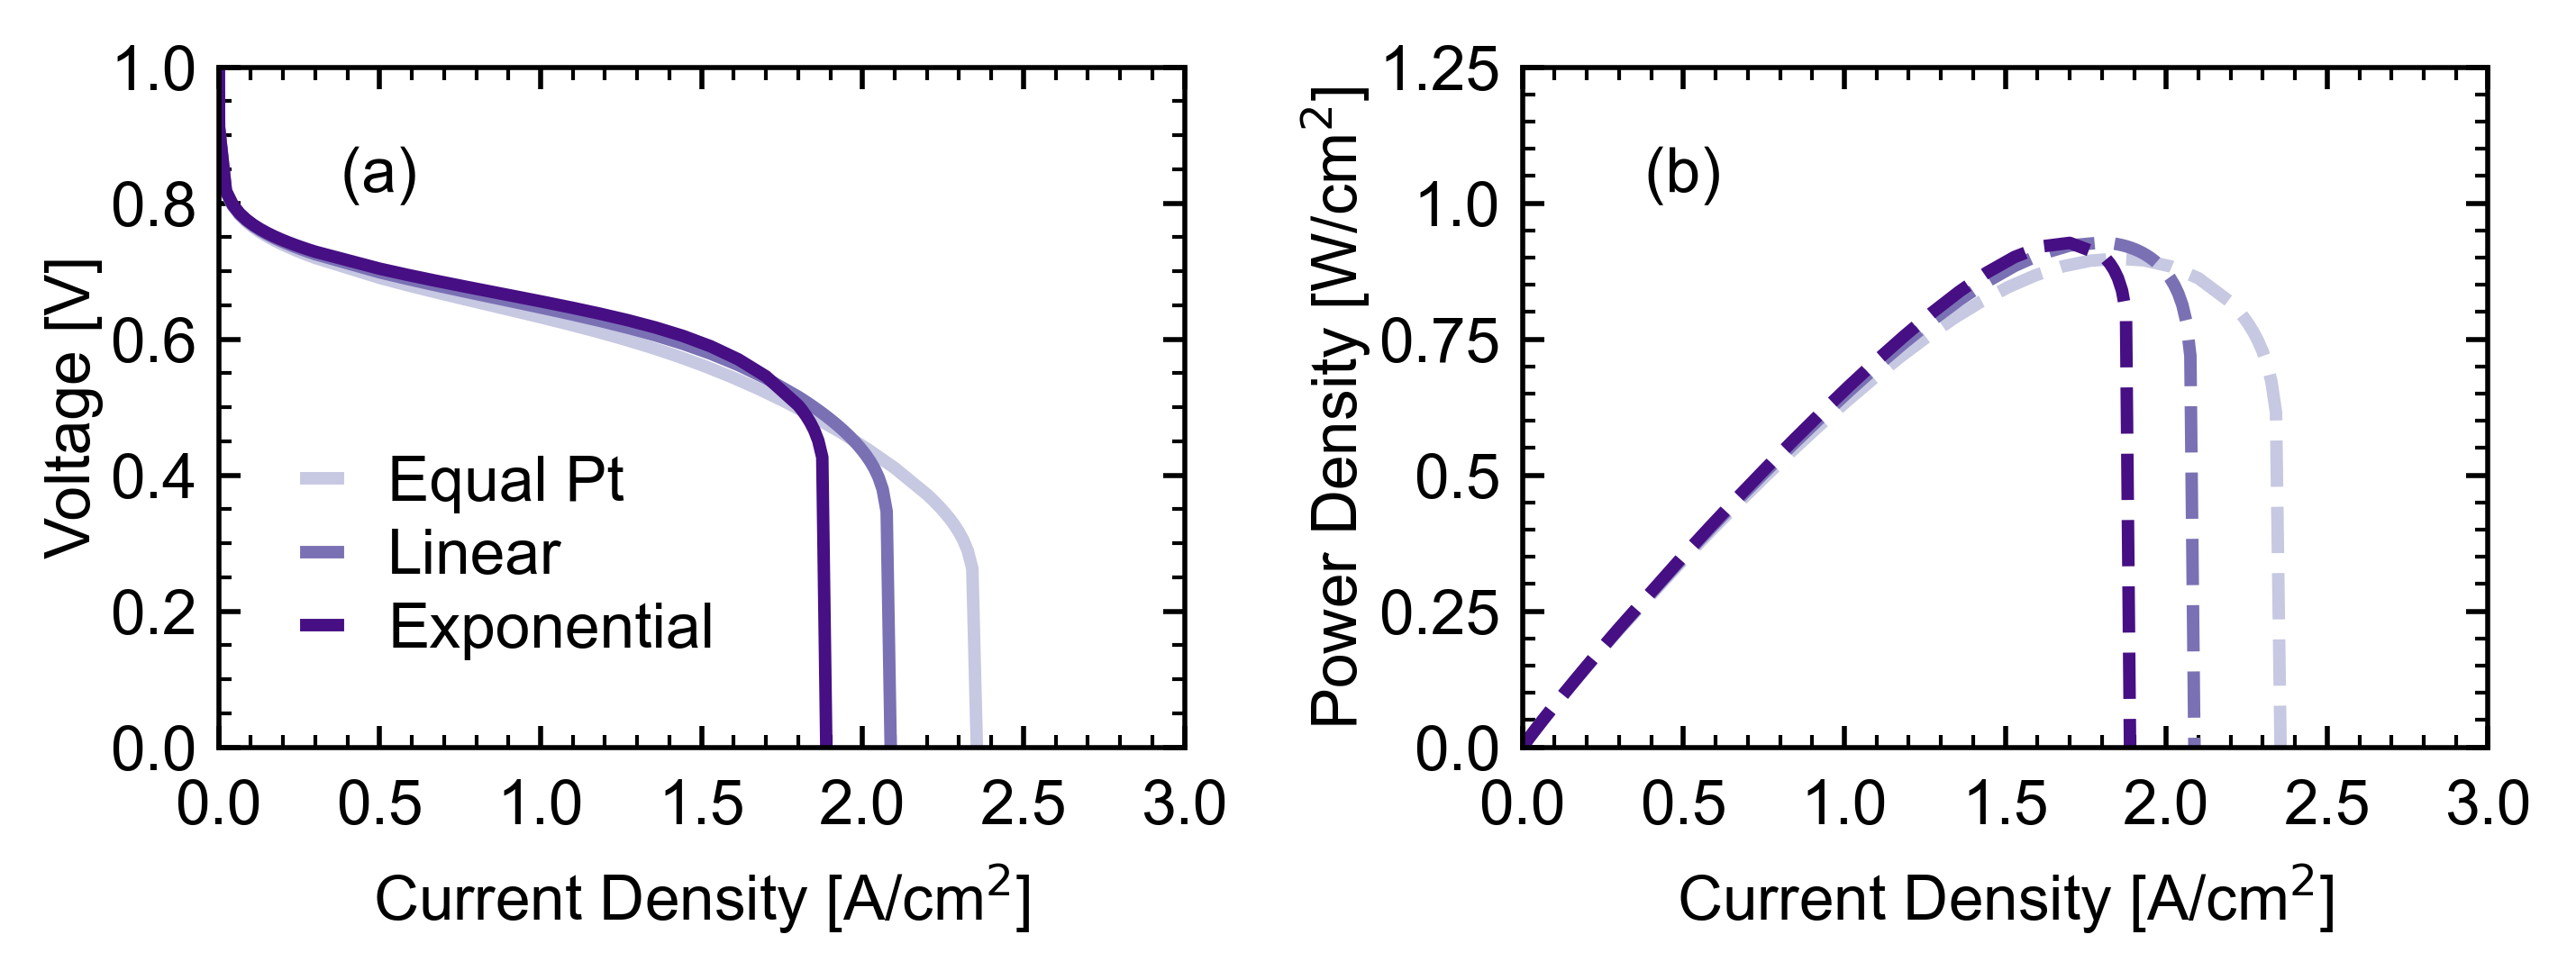
\includegraphics[width=5.718in]{figures/pt-distribution-5_718in.png}
    \caption{(a) Polarization and (b) power density curves for varying Pt distributions. The curves labeled ``Equal Pt'' are for the model validation base case where the Pt is evenly distributed. Results suggest marginal improvements to power density for the graded Pt distributions at a significant cost of lower limiting currents.}
    \label{fig:Pt-distribution-study}
\end{figure}
As shown in Figure~\ref{fig:dual-graded}, combining graded Pt loadings with graded Nafion loadings to mitigate flooding effects provides a pathway to low-Pt PEMFCs with superior performance.  Such `dual graded' CL designs improved both the maximum power density \emph{and} the limiting current, relative to all other CL designs consiered. 


% References
\bibliographystyle{unsrt}
\bibliography{bibliography}

\end{document}